\chapter*{Dodatak: Prikaz aktivnosti grupe}
		\addcontentsline{toc}{chapter}{Dodatak: Prikaz aktivnosti grupe}
		
		\section*{Dnevnik sastajanja}
		
		\textbf{\textit{Kontinuirano osvježavanje}}\\
		
		 \textit{U ovom dijelu potrebno je redovito osvježavati dnevnik sastajanja prema predlošku.}
		
		\begin{packed_enum}
			\item  sastanak
			
			\item[] \begin{packed_item}
				\item Datum: 19. listopada 2023.
				\item Prisustvovali: Dominik Dejanović, Ante Čavar, Borna Dramalija, Adam Vuković, Nikola Trebus, Ljubica Nikolić
				\item Teme sastanka:
				\begin{packed_item}
					\item  upoznavanje tima
					\item  raspodjela zadataka
					\item rasprava o korištenim tehnologijama
				\end{packed_item}
			\end{packed_item}
			
			\item  sastanak
			\item[] \begin{packed_item}
				\item Datum: 27. listopada 2023.
				\item Prisustvovali: Dominik Dejanović, Ante Čavar, Adam Vuković, Nikola Trebus, Ante Volarević, Ljubica Nikolić
				\item Teme sastanka:
				\begin{packed_item}
					\item  dogovor oko dizajna baze podataka
					\item  dogovor oko rada na dokumentaiciji
					\item rasprava o budućim ciljevima
				\end{packed_item}
			\end{packed_item}
			
			
			\item  sastanak
			\item[] \begin{packed_item}
				\item Datum: 2. studeni 2023.
				\item Prisustvovali: Ljubica Nikolić, Ante Čavar
				\item Teme sastanka: 
				\begin{packed_item}
					\item izrada dokumentacije
					\item izrada osnovne verzije API-a
				\end{packed_item}
			\end{packed_item}
			
			\item  sastanak
			\item[] \begin{packed_item}
				\item Datum: 9. listopada 2023.
				\item Prisustvovali: Dominik Dejanović, Ljubica Nikolić
				\item Teme sastanka:
				\begin{packed_item}
					\item izrada početne web stranice
					\item razdijela stranica za prijavu i registraciju
					\item dokumentacija - UML i sekvencijski dijagrami
				\end{packed_item}
			\end{packed_item}
			
			\item  sastanak
			\item[] \begin{packed_item}
				\item Datum: 14. listopada 2023.
				\item Prisustvovali: Dominik Dejanović, Ante Čavar, Adam Vuković, Nikola Trebus, Ljubica Nikolić, Ante Volarević
				\item Teme sastanka:
				\begin{packed_item}
					\item raspodijela zadataka
					\item razgovor o deployanju stranice
				\end{packed_item}
			\end{packed_item}
			
			\item  sastanak
			\item[] \begin{packed_item}
				\item Datum: 16. listopada 2023.
				\item Prisustvovali: Dominik Dejanović, Ante Čavar, Adam Vuković, Nikola Trebus, Ante Volarević
				\item Teme sastanka:
				\begin{packed_item}
					\item raspodijela završnih zadataka
				\end{packed_item}
			\end{packed_item}
			\item  sastanak
            \item[] \begin{packed_item}
                \item Datum: 7. prosinca 2023.
            \item Prisustvovali: Dominik Dejanović, Ante Čavar
                \item Teme sastanka:
                \begin{packed_item}
                    \item osvrt na prvi ciklus
                \end{packed_item}
            \end{packed_item}


            \item  sastanak
            \item[] \begin{packed_item}
                \item Datum: 21. prosinca 2024.
                \item Prisustvovali: Dominik Dejanović, Ante Čavar, Adam Vuković, Nikola Trebus, Ante Volarević, Ljubica Nikolić
                \item Teme sastanka: 
                \begin{packed_item}
                    \item budući rad kao šesteročlana grupa
                \end{packed_item}
            \end{packed_item}

            \item  sastanak
            \item[] \begin{packed_item}
                \item Datum: 11. siječnja 2024.
                \item Prisustvovali: Dominik Dejanović, Ante Čavar, Adam Vuković, Nikola Trebus, Ante Volarević, Ljubica Nikolić
                \item Teme sastanka:
                \begin{packed_item}
                    \item raspodjela preostalog posla
                \end{packed_item}
            \end{packed_item}

            \item  sastanak
            \item[] \begin{packed_item}
                \item Datum: 19. siječnja 2024.
                \item Prisustvovali: Dominik Dejanović, Ante Čavar, Adam Vuković, Nikola Trebus, Ljubica Nikolić, Ante Volarević
                \item Teme sastanka:
                \begin{packed_item}
                    \item troubleshooting
                    \item završne promjene
                \end{packed_item}
            \end{packed_item}
			
			%
			
		\end{packed_enum}
		
		\eject
		\section*{Tablica aktivnosti}
		
			%\textbf{\textit{Dokumentacija}}\\
			Aktivnost izražena u satima.

			\begin{longtblr}[
					label=none,
				]{
					vlines,hlines,
					width = \textwidth,
					colspec={X[7, l]X[1, c]X[1, c]X[1, c]X[1, c]X[1, c]X[1, c]X[1, c]}, 
					vline{1} = {1}{text=\clap{}},
					hline{1} = {1}{text=\clap{}},
					rowhead = 1,
				} 
			
				\SetCell[c=1]{c}{} & \SetCell[c=1]{c}{\rotatebox{90}{\textbf{Dominik Dejanović}}} & \SetCell[c=1]{c}{\rotatebox{90}{\textbf{Adam Vuković}}} &	\SetCell[c=1]{c}{\rotatebox{90}{\textbf{Ljubica Nikolić}}} & \SetCell[c=1]{c}{\rotatebox{90}{\textbf{Ante Volarević }}} &	\SetCell[c=1]{c}{\rotatebox{90}{\textbf{Nikola Trebus }}} & \SetCell[c=1]{c}{\rotatebox{90}{\textbf{Ante Čavar }}} \\  
				Upravljanje projektom 		& 2  &  &  &  &  &  & \\ 
				Opis projektnog zadatka 	&  &  3  &  &  &  & \\ 
				
				Funkcionalni zahtjevi       &  &  & 2  &  &  &  &  \\ 
				Opis pojedinih obrazaca 	& 4  &  & 2  &  &  &  &  \\ 
				Dijagram obrazaca 			& 1  &  & 3  &1  &  &  &  \\ 
				Sekvencijski dijagrami 		& 1  &  & 7  &  &  &  &  \\ 
				Opis ostalih zahtjeva 		&  &  & 5 &  &  &  &  \\ 

				Arhitektura i dizajn sustava	 & 3 &  &  &  & 2 & 1 &  \\ 
				Baza podataka				&  & 1 & 2 & 1 & 1 & 6 &   \\ 
				Dijagram razreda 			&  &  & 30 &  & 15 &  &   \\ 
				Dijagram stanja				&  & 4 &  &  &  &  &  \\ 
				Dijagram aktivnosti 		&  & 3 &  &  &  &  &  \\ 
				Dijagram komponenti			&  & 3 &  &  &  &  &  \\ 
				Korištene tehnologije i alati 		&  &  & 2 &  &  &  &  \\ 
				Ispitivanje programskog rješenja 	& 10 &  &  &  &  & 15 &  \\ 
				Dijagram razmještaja			&  & 2 &  &  &  &  &  \\ 
				Puštanje u pogon 		& 10 &  &  & 2 &  & 10 &  \\  
				Dnevnik sastajanja 			& 1  &  &  &  & 2 &  &  \\ 
				Zaključak i budući rad 		&  &  &  &  &  & 1 &  \\  
				Popis literature 			&  &  &  &  &  &  &  \\  
				Web stranica & 12 & 35 &  &  &  &  & \\
				&  &  &  &  &  &  &  \\ \hline 
				\textit{Dodatne stavke kako ste podijelili izradu aplikacije} 			&  &  &  &  &  &  &  \\ 
				\textit{npr. izrada početne stranice} 				&  &  &  &  &  &  &  \\  
				\textit{izrada baze podataka} 		 			&  & 2 &  & 1 &  &  & \\  
				\textit{spajanje s bazom podataka} 							&  & 2 &  & 1 &  &  &  \\ 
				\textit{back end} 							& 5 & 10 &  & 6 & 3 & 30 &  \\  
				 							&  &  &  &  &  &  &\\ 
			\end{longtblr}
					
					
		\eject
		\section*{Dijagrami pregleda promjena}
		
		\textbf{\textit{dio 2. revizije}}\\
		
		\textit{Prenijeti dijagram pregleda promjena nad datotekama projekta. Potrebno je na kraju projekta generirane grafove s gitlaba prenijeti u ovo poglavlje dokumentacije. Dijagrami za vlastiti projekt se mogu preuzeti s gitlab.com stranice, u izborniku Repository, pritiskom na stavku Contributors.}
		
		
			\begin{figure}[H]\centering
				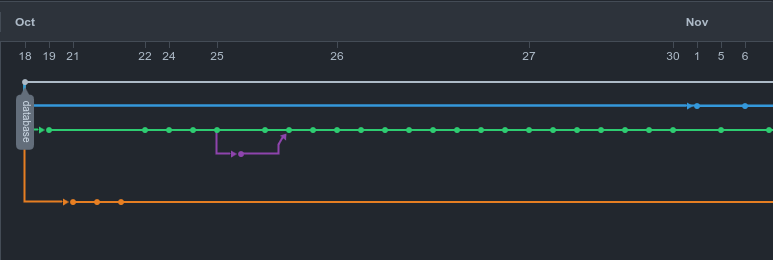
\includegraphics[width=1\textwidth]{slike/image.png}
				\caption{}
			\end{figure}
			
			\begin{figure}[H]\centering
				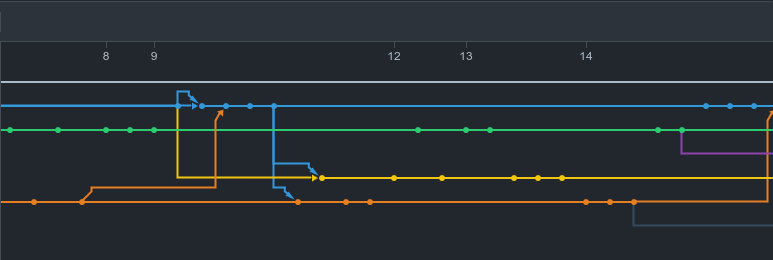
\includegraphics[width=1\textwidth]{slike/image2.png}
				\caption{}
			\end{figure}
			 
			\begin{figure}[H]\centering
				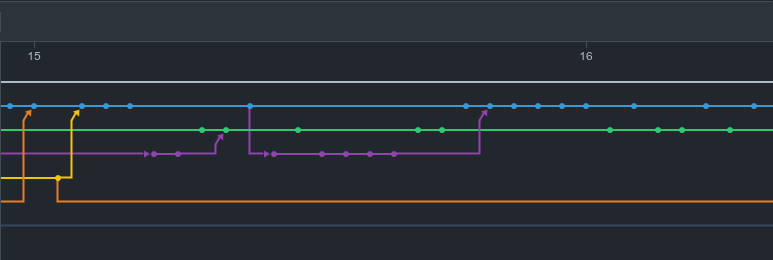
\includegraphics[width=1\textwidth]{slike/image3.png}
				\caption{}
			\end{figure}
		
			\begin{figure}[H]\centering
				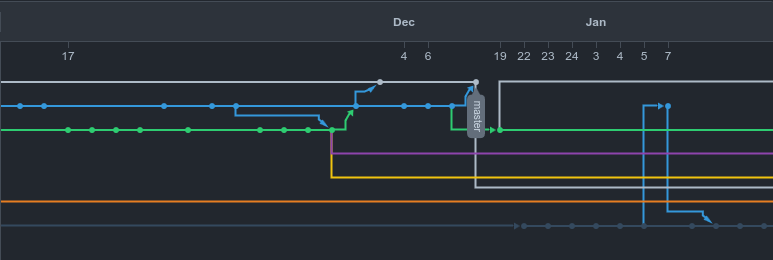
\includegraphics[width=1\textwidth]{slike/image4.png}
				\caption{}
			\end{figure}
			
			\begin{figure}[H]\centering
				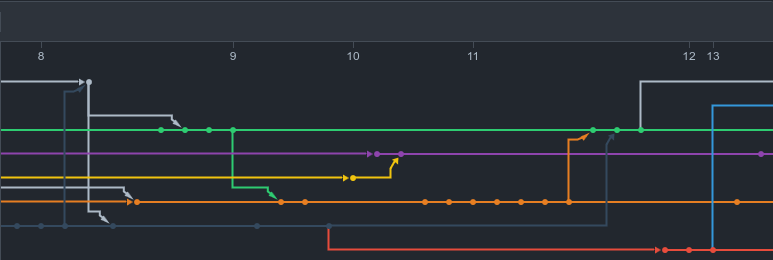
\includegraphics[width=1\textwidth]{slike/image5.png}
				\caption{}
			\end{figure}
	
			\begin{figure}[H]\centering
				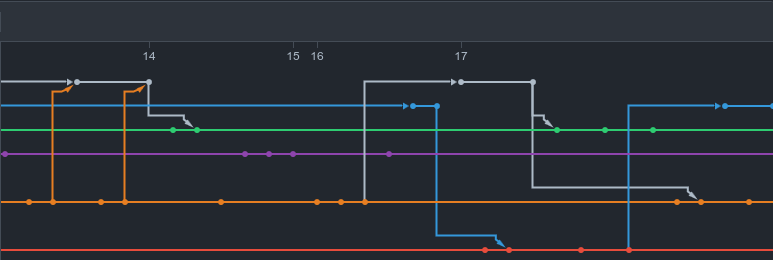
\includegraphics[width=1\textwidth]{slike/image6.png}
				\caption{}
			\end{figure}
		
			\begin{figure}[H]\centering
				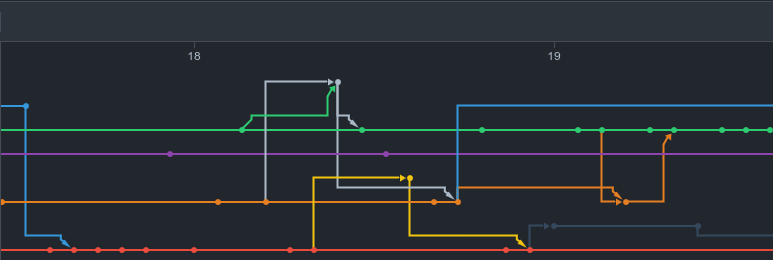
\includegraphics[width=1\textwidth]{slike/image7.png}
				\caption{}
			\end{figure}
			
			\begin{figure}[H]\centering
				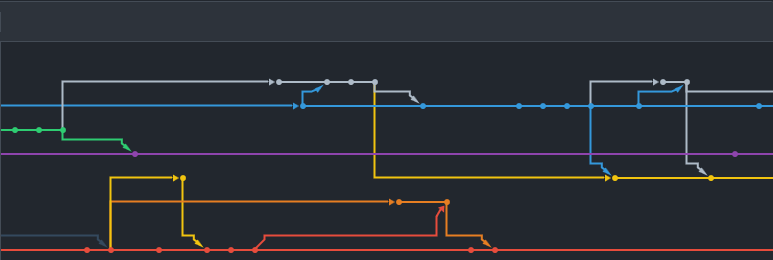
\includegraphics[width=1\textwidth]{slike/image8.png}
				\caption{}
			\end{figure}
		